\documentclass[a4paper,10pt,standalone]{book}
\usepackage[T1]{fontenc}
%\usepackage[utf8]{inputenc}
\usepackage{lmodern,amsmath,amsfonts,amssymb,amsthm,graphicx,color,xcolor,url,theorem,textcomp,glossaries,parskip,xlop,multicol,calculator,hyperref,tikz,fontspec,mathpazo, setspace}
%\doublespacing
%\onehalfspacing
\usepackage{unicode-math}
%\defaultfontfeatures{Numbers=Lining}
\setmainfont{xkcd Script}
\setmathfont{xkcd Script}
\usetikzlibrary{decorations.pathreplacing,calligraphy,decorations.pathmorphing,calc,positioning,intersections,external}
\tikzexternalize[prefix=figures/]
\usepackage [english]{babel}
\usepackage [autostyle, english = american]{csquotes}
\MakeOuterQuote{"}
\graphicspath{ {./Images/} }

\raggedright
\newcommand{\subchapter}[5]{
%\if\relax\detokenize{#1}\relax
%\phantom{I}\newline
%\else \textnormal{(#1)}%
%\fi
%\if\relax\detokenize{#2}\relax
%\phantom{I}\newline
%\else \textnormal{(#2)}%
%\fi
%\if\relax\detokenize{#3}\relax
%\phantom{I}\newline
%\else \textnormal{(#3)}%
%\fi
%\if\relax\detokenize{#4}\relax
%\phantom{I}\newline
%\else \textnormal{(#4)}%
%\fi
%\if\relax\detokenize{#5}\relax
%\phantom{I}\newline
%\else \textnormal{(#5)}%
%\fi

\begin{multicols*}{2}
\raggedcolumns
\section{#1}
\vfill
\subsection*{} #2
\vfill
\subsection*{Solution} #3
\vfill
\subsection*{Definition} #4
 \columnbreak
 \subsection*{}
\begin{center}
\vspace*{\fill}
    #5
    \vspace*{\fill}
\end{center}
\end{multicols*}
\vfill
\pagebreak
}

\title{\textbf{Duckie}\linebreak \textit{And The Search For The Golden Goose}}
\date{}
\author{Iniyan Joseph}

\begin{document}
\maketitle
\newcommand{\distanceOneOpO}{3}
\newcommand{\distanceTwoOpO}{4}
\ADD{\distanceOneOpO}{\distanceTwoOpO}{\distanceThreeOpO}
\newcommand{\distanceFourOpTw}{3}
\MULTIPLY{\distanceThreeOpO}{\distanceFourOpTw}{\distanceFiveOpTw}
\newcommand{\distanceSixOpTh}{-3}
\ABSVALUE{\distanceSixOpTh}{\distanceSixAbsOpTh}
\ADD{\distanceFiveOpTw}{\distanceSixOpTh}{\distanceSevenOpTh}
\newcommand{\distanceEightOpFo}{-6}
\ABSVALUE{\distanceEightOpFo}{\distanceEightAbsOpFo}
\SUBTRACT{\distanceSevenOpTh}{\distanceEightOpFo}{\distanceNineOpFi}
%\chapter*{Introduction}     
%\section*{Why Write this Book}

%\paragraph*{} Mathematics is an essential aspect of human life. There is a stereotype of people disliking and struggling with mathematics, which I believe is simply because we are, at a young age, often told to try to compute, rather than being challenged with fundamental questions of how to understand the world around us. 
%\section*{How to use this book}
%\paragraph*{} Learning and understanding mathematics takes more than reading this book purely for its story, but wrestling with new ideas and questions, and attempting to resolve those questions through reasoning. To this end, after reading the story on each page, have students attempt to develop an answer using their intuition and prior knowledge to build toward the correct answer. Only after they have worked towards the right answer without hints and engaged in discussion, read the solution.
%\paragraph{} Even beyond the scope of the book, encourage them to ask questions about the world around them. Reason through math in games they know and love, in stories, and in everyday life and present unintuitive problems which they can use the tools from this book and otherwise to solve in genuine scenarios. 
%\section*{Additional Resources} 
%\begin{itemize}
%\item MathForLove \url{https://mathforlove.com/}
%\item MathIsFun \url{https://www.mathsisfun.com/}
%\end{itemize}

\tableofcontents
\vfill
\pagebreak
%Introduce the story
\paragraph{} All was quiet in the goose village. The cool autumn breeze scented the air with pine, and shuffled the dry leaves across the forest floor. The sun shone brightly and warmly, casting light on the main path. To an outsider looking at the village, with the older geese talking with one another and the goslings running around playing, it would have seemed an idyllic life. Undoubtedly, it was a sort of place where parent geese could look out and feel their goslings were safe. At any other time, it would have been a pleasant evening - a tranquil picture of happiness. Yet that fall evening, there was a sense of despair in the village. Each goose knew that their quiet evenings would soon be over, and that they would have to leave for migration. 
\paragraph{} "Enough is enough." Duckie thought. For as long as he could remember, he had been afraid of the long journey. With the icy mountain peaks and vast exposing stretches of forest, the journey left him and the other geese vulnerable to the unwelcome dangers of the wilderness. The vulnerability of the long travel was compounded by the harsh environment. Duckie looked up the main road at city hall, where the goose authorities stood watching the city. 
\paragraph{} Created to protect the village from danger, the goose authorities created and enforced the rules village. To ensure the the citizens followed their rules, they created the elite corps of goose police. This system had worked for some time, but in the past years, they had abused their power. They had closed down the schools, burned the village's books, and closed off the village from the outside world. But what could he do? The goose authorities, the leaders of the village, had controlled migrations for as long as anyone in the village could remember, and he would soon have to embark on the dangerous journey.
\paragraph{} Growing up, Duckie had heard the stories of the fabled "golden goose" of legend who lived on the highest mountain. According to the stories, the golden goose would bring great change to the village. That change would in turn lead to great change, and would save the village from tyranny, and lead to an era of peace. Many geese had tried to seek her, but it was a dangerous journey, and none had ever returned. 
\paragraph{} "No. I have no choice." 
\paragraph{} Duckie thought back to his childhood. In large part, it had been a quiet life. To most people, it seemed completely average, but he had had the opportunity to find some great mentors. He thought back to the faraway place on the grassy mound, where he used to meet with the wise old goose who lived outside the village. He remembered the goose's last words before leaving for his last cold winter's migration.
\paragraph{} "Remember the legend Duckie. Remember the golden goose." 
\vfill
\pagebreak
\chapter{Arithmetic}
\paragraph{} That night, Duckie decided to leave the village. He knew he would leave secretly because of the tyrannical rules of the goose authorieties. They had tried so hard to keep their power, and the search for the Golden Goose risked everything they stood for. Duckie waited until everyone had gone to sleep, and started on his journey.
\paragraph{} He began to sneak towards the village border, where he saw two guards snoring loudly. He tiptoed past, and all seemed quiet, but just as he turned his back to the village, he heard alarms ringing. 
\paragraph{} \textbf{Honk! Honk! Honk!}
\paragraph{} They droned. Duckie turned around and saw the two guards he had walked past coming towards him. The goose authorities had been alerted of his mission, and he would have to run. He began flying, and as he looked back, saw the goose police on his tail. 
\vfill
\pagebreak
%Addition
\subchapter{Addition}
{On the first night of his journey, Duckie flew $\mathbf{3} km$ from the village towards the mountain with the goose police in pursuit. Looking back, he wouldn't see them behind him, so, unsure of how far the goose police would chase him, he decided to take a quick break to gain his strength, but in a flash, he saw the police on the horizon and began to fly again. From there, he flew another $\mathbf{4} km$. Duckie wanted to know how much he had traveled in the direction of the mountain. Where was Duckie?}
{He first flew $\mathbf{3} km$, then changed this amount by $\mathbf{4}$. Duckie's position, 3 kilometers, changed by 4 kilometers. This is $\opadd{3}{4} km$.}
{Addition, or adding, is the most basic way of using numbers. It represents changing one number by another to form a single, combined number.} 
{\begin{tikzpicture}
    \coordinate (A) at (0,0);
    \coordinate (B) at (0,\distanceOneOpO);
    \coordinate (C) at (0,\distanceTwoOpO);

   \node [inner sep=0pt] at (C) {
\includegraphics[height=0.8cm]{DuckieGami}};
    \draw[->,ultra thick,red, decorate, decoration={random steps,segment length=3pt,amplitude=0.2pt}] (A) -- (B) node[midway, left] {$\distanceOneOpO km$};
    \draw[->,ultra thick,blue, decorate, decoration={random steps,segment length=3pt,amplitude=0.2pt}] (B) -- (C) node[midway, left] {$\distanceTwoOpO km$};

    \draw [decorate,
	decoration = {calligraphic brace,mirror,
		raise=10pt,amplitude=5pt}] (A) -- (C) node[midway, right, xshift=0.5cm,line width=3pt] {$\distanceThreeOpO km$};
\end{tikzpicture}
}
%Multiplication
\subchapter{Multiplication}
{As Duckie began his journey towards the mountain, the goose authorities followed close behind. Every time he turned back, he saw them on the horizon. On each of the first three days, he flew $\mathbf{7km}$. Duckie wanted to know how much he had flown towards the mountain. Where was Duckie?}
{Duckie flew $\mathbf{7} km$, $\mathbf{3} times$. This means the amount he flew was triple what he flew on the first day. This is $\opmul{3}{7} km$.}
{Multiplication, or multiplying, is the second basic way of using numbers. It represents changing a number by a certain scale. For example, doubling, tripling, etc. $A\ast B$ is $A$ times more than $B$.}
{ \begin{tikzpicture}
    \coordinate (A) at (0,0);
    \coordinate (B) at (0,3);
    \coordinate (C) at (0,6);
    \coordinate (D) at (0,9);

    \node [inner sep=0pt] at (D) {
\includegraphics[height=0.8cm]{DuckieGami}};
    \draw[->,ultra thick,red, decorate, decoration={random steps,segment length=3pt,amplitude=0.2pt}] (A) -- (B) node[midway, left] {$7 km$};
    \draw[->,ultra thick,blue, decorate, decoration={random steps,segment length=3pt,amplitude=0.2pt}] (B) -- (C) node[midway, left] {$7 km$};
    \draw[->,ultra thick,violet, decorate, decoration={random steps,segment length=3pt,amplitude=0.2pt}] (C) -- (D) node[midway, left] {$7 km$};

    \draw [decorate,
	decoration = {calligraphic brace,mirror,
		raise=10pt,amplitude=5pt}] (A) -- (D) node[midway, right, xshift=0.5cm,line width=3pt] {$21 km$};
\end{tikzpicture}
}
%Negatives
\subchapter{Negative Numbers}
{On the morning of the fourth day, Duckie had traveled $\mathbf{21} km$. He decided he had to take evasive maneuvers to try to confuse the goose police. Their training to be the fastest and best in the village meant they would inevitably catch up with him. To escape, he decided do the last thing they expected: go back towards the village. He traveled in the opposite direction of the mountain for $\mathbf{3} km$. Duckie wanted to know how far he was from the mountain. Where was Duckie?}
{This is called $\mathbf{-3} km$. \linebreak – means opposite direction.  He first flew $\mathbf{21} km$, then flew $\mathbf{-3} km$. This is$ \opsub{21}{3} km$.}
{A number less than 0 is called "negative", and is in the opposite direction.}
{\begin{tikzpicture}
    \coordinate (A) at (0,0);
    \coordinate (B) at (0,9);
    \coordinate (C) at (1,9);
    \coordinate (D) at (1,8);
    \coordinate (E) at (2,0);
    \coordinate (F) at (2,8);

    \node [inner sep=0pt] at (F) {
\includegraphics[height=0.8cm]{DuckieGami}};
    \draw[->,ultra thick,red, decorate, decoration={random steps,segment length=3pt,amplitude=0.2pt}] (A) -- (B) node[midway, right] {$21 km$};
    \draw[->,ultra thick,blue, decorate, decoration={random steps,segment length=3pt,amplitude=0.2pt}] (C) -- (D) node[midway, right] {$-3 km$};
    \draw[->,ultra thick,violet, decorate, decoration={random steps,segment length=3pt,amplitude=0.2pt}] (E) -- (F) node[midway, right] {$18 km$};
\end{tikzpicture}
}
%Multiples of a negative
\subchapter{Multiples of a negative}
{Duckie was tried from traveling so much in the past few days. As he traveled in the negative direction, to try to gain his strength for the difficult journey ahead, he took a break every $\mathbf{-1} km$. He flew that distance $\mathbf{3}$ times. How far did Duckie travel while taking evasive maneuvers?}
{Duckie traveled $\mathbf{-1} km$ $\mathbf{3}$ times. This is -$\opmul{3}{1}$ km}
{Multiplying by a negative number shows stretching or scaling a number by some amount, but in the opposite direction.}
{ \begin{tikzpicture}
    \coordinate (A) at (0,0);
    \coordinate (B) at (0,9);
    \coordinate (C) at (1,9);
    \coordinate (D) at (1,8.666);
    \coordinate (E) at (1,8.333);
    \coordinate (F) at (1,8);
    \coordinate (G) at (2,0);
    \coordinate (H) at (2,8);

    \node [inner sep=0pt] at (H) {
\includegraphics[height=0.8cm]{DuckieGami}};
    \draw[->,ultra thick,red, decorate, decoration={random steps,segment length=3pt,amplitude=0.2pt}] (A) -- (B) node[midway, right] {21 km};
    \draw[->,ultra thick,blue, decorate, decoration={random steps,segment length=3pt,amplitude=0.2pt}] (C) -- (D) node[midway, right] {-1};
    \draw[->,ultra thick,blue, decorate, decoration={random steps,segment length=3pt,amplitude=0.2pt}] (D) -- (E) node[midway, right] {-1};
    \draw[->,ultra thick,blue, decorate, decoration={random steps,segment length=3pt,amplitude=0.2pt}] (E) -- (F) node[midway, right] {-1};
     \draw[->,ultra thick,violet, decorate, decoration={random steps,segment length=3pt,amplitude=0.2pt}] (G) -- (H) node[midway, right] {18 km};
\end{tikzpicture}
}
%Negative of a Negative
\subchapter{Negative of a Negative}
{On the fifth day, feeling that he had avoided the goose police and confused them, continued to head towards the mountain. To get to the Golden Goose, he knew he would have to travel away from the village, and so turned around and flew for $\mathbf{6} km$. Duckie traveled in the opposite direction of the negative direction by $\mathbf{6}$, or $\mathbf{-(-6)}$. Duckie wanted to know how far he was from the mountain. Where was Duckie?}
{Initially, Duckie was at $\mathbf{18 km}$. He then traveled $\mathbf{-(-6)}$. Duckie traveled $\mathbf{6} km$ towards the mountain. he had flown $\opadd{18}{6} km$ towards the mountain.}
{The opposite direction of the opposite or negative direction of a number is in the same direction of the number. It is written as -(-number), which is the same as the number itself.}
{ \begin{tikzpicture}
    \coordinate (A) at (0,0);
    \coordinate (B) at (0,6);
    \coordinate (C) at (1,0);
    \coordinate (D) at (1,-6);
    \coordinate (E) at (2,0);
    \coordinate (F) at (2,6);

    \node [inner sep=0pt] at (F) {
\includegraphics[height=0.8cm]{DuckieGami}};
    \draw[->,ultra thick,red, decorate, decoration={random steps,segment length=3pt,amplitude=0.2pt}] (A) -- (B) node[midway, right] {6 km};
    \draw[->,ultra thick,blue, decorate, decoration={random steps,segment length=3pt,amplitude=0.2pt}] (C) -- (D) node[midway, right] {-6 km};
    \draw[->,ultra thick,violet, decorate, decoration={random steps,segment length=3pt,amplitude=0.2pt}] (E) -- (F) node[midway, right] {- -6 km};
\end{tikzpicture}
}
%Multiplication Table
\section{Multiplication Table}
\begin{table}[h]
\centering
\begin{tabular}{c| llllllllllll}
   & 0          & 1          & 2          & 3          & 4           & 5           & 6           & 7           & 8           & 9           & 10            \\
   \hline
0  & \textbf{0} & 0          & 0          & 0          & 0           & 0           & 0           & 0           & 0           & 0           & 0             \\
1  & 0          & \textbf{1} & 2          & 3          & 4           & 5           & 6           & 7           & 8           & 9           & 10            \\
2  & 0          & 2          & \textbf{4} & 6          & 8           & 10          & 12          & 14          & 16          & 18          & 20            \\
3  & 0          & 3          & 6          & \textbf{9} & 12          & 15          & 18          & 21          & 24          & 27          & 30            \\
4  & 0          & 4          & 8          & 12         & \textbf{16} & 20          & 24          & 28          & 32          & 36          & 40            \\
5  & 0          & 5          & 10         & 15         & 20          & \textbf{25} & 30          & 35          & 40          & 45          & 50            \\
6  & 0          & 6          & 12         & 18         & 24          & 30          & \textbf{36} & 42          & 48          & 54          & 60            \\
7  & 0          & 7          & 14         & 21         & 28          & 35          & 42          & \textbf{49} & 56          & 63          & 70            \\
8  & 0          & 8          & 16         & 24         & 32          & 40          & 48          & 56          & \textbf{64} & 72          & 80            \\
9  & 0          & 9          & 18         & 27         & 36          & 45          & 54          & 63          & 72          & \textbf{81} & 90            \\
10 & 0          & 10         & 20         & 30         & 40          & 50          & 60          & 70          & 80          & 90          & \textbf{100} 
\end{tabular}
\end{table}
\paragraph{Observations about the Multiplication Table}:
\linebreak
\paragraph{0} Any number multiplied by 0 is 0. This makes sense, because any number
repeated 0 times is the same as not having it at all.
\paragraph{1} Any number multiplied by 1 is itself. This makes sense, because any
number repeated one time is itself. This has a special name: \textit{Identity}
\paragraph{10} Any number multiplied by 10 is shifted to the left by one digit.
\paragraph{Symmetry} The table is identical across the diagonal. This shows
that 4$\ast$2 is the same as 2$\ast$4. This property also has a special name:
\textit{Commutativity}.
\chapter{Properties}
\paragraph{} After five days of running from the goose police, Duckie was certain that he had escaped. He decided to stop and eat dinner, but just as he began to land, \textbf{Squawk!} He ran headfirst into another goose. 
\paragraph{} "Hold it right there! You need to come back with me to the village!" the policegoose demanded, slightly dazed. 
\paragraph{} "It's dangerous in the outside world. This is for your own safety!"
\paragraph{} Duckie knew that the policegoose, named Güs was rational and decided to try to reason with him. "Of course it's dangerous! But I have to do this. I am looking for the golden goose of legend. The one who is supposed to save us, change all of goose society and help us through our migrations."
\paragraph{} "But that's against the rules! Why would you risk your life to break their rules? Don't they keep us safe?" Güs asked.
\paragraph{} "Its true. Some of the rules do keep us same, but too many take away our liberty. I think they are afraid of what will happen if I find the golden goose. If I can find her, then they may not be able to stay in power. You joined the goose police to help people, and if you let me go, you can do just that!"
\paragraph{} "You might be right, but I can't betray the village. If I just let you go without at least trying to stop you, I won't be able to look myself in the mirror, much less be seen in the village! I have no interest in fighting, so I'll tell you what. I will have a set of challenges with you. If you beat me, I will let you go. If not, you have to let me take you back. Sound fair?"
\paragraph{} Duckie was reluctant, but knew that he had no other options. "Fine. Let's do the challenges."
\pagebreak
\subchapter{Associativity}
{Güs and Duckie both felt that they were good fliers. 
\paragraph{} "To begin, let's do a flying contest in 3 parts." Gus announced. "Whoever flies the furthest wins."
\paragraph{} Duckie thought about this. "Fine, but to make sure no one gets an unfair advantage, let's allow one break in between."
\paragraph{} The first leg of the race was $1 km$, the second leg was $\mathbf{2} km$, and the third leg was $\mathbf{1} km$. Duckie and Güs both wanted to win, so created strategies. Güs decided to travel the first leg ($\mathbf{1} km$) of the race, took his break then travel the second and third legs ($\mathbf{2} km$ and $\mathbf{1} km$). Duckie instead traveled the first leg, ($\mathbf{1} km$) of the race and the second leg ($\mathbf{2} km$) of the race, then took his break, and traveled the third leg ($\mathbf{1} km$). Did they tie by traveling the same amount?}
{Yes! Duckie traveled $(\mathbf{1} km + \mathbf{2} km) + \mathbf{3} km = \mathbf{5} km$. Güs traveled $\mathbf{1} km + (\mathbf{2} km + \mathbf{3} km) = \mathbf{5}km$. Duckie and Güs both traveled $\mathbf{5km}$.}
{Adding can be grouped in any way. In other words: (A+B)+C = A+(B+C).}
{\begin{tikzpicture}
    \coordinate (A) at (0,0);
    \coordinate (B) at (0,2);
    \coordinate (C) at (0,6);
    \coordinate (D) at (0,8);
    \coordinate (Ap) at (1.5,0);
    \coordinate (Bp) at (1.5,2);
    \coordinate (Cp) at (1.5,6);
    \coordinate (Dp) at (1.5,8);

    \node [inner sep=0pt] at (D) {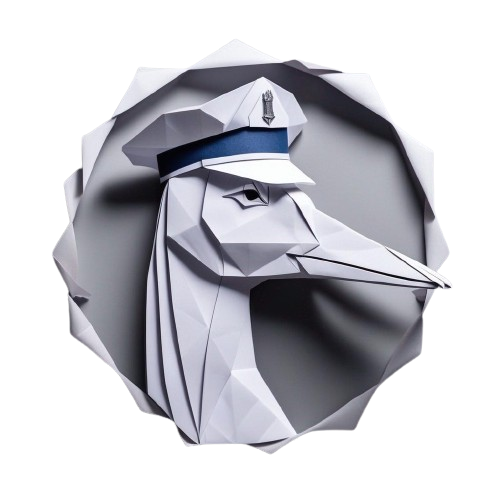
\includegraphics[height=0.8cm]{Gus}};
    \draw[-|,ultra thick,red, decorate, decoration={random steps,segment length=3pt,amplitude=0.2pt}] (A) -- (B) node[midway, left] {$1 km$};
    \draw[->,ultra thick,blue, decorate, decoration={random steps,segment length=3pt,amplitude=0.2pt}] (B) -- (C) node[midway, left] {$2 km$};
    \draw[->,ultra thick,violet, decorate, decoration={random steps,segment length=3pt,amplitude=0.2pt}] (C) -- (D) node[midway, left] {$1 km$};

    \node [inner sep=0pt] at (Dp) {
\includegraphics[height=0.8cm]{DuckieGami}};
    \draw[->,ultra thick,red, decorate, decoration={random steps,segment length=3pt,amplitude=0.2pt}] (Ap) -- (Bp) node[midway, left] {$1 km$};
    \draw[-|,ultra thick,blue, decorate, decoration={random steps,segment length=3pt,amplitude=0.2pt}] (Bp) -- (Cp) node[midway, left] {$2 km$};
    \draw[->,ultra thick,violet, decorate, decoration={random steps,segment length=3pt,amplitude=0.2pt}] (Cp) -- (Dp) node[midway, left] {$1 km$};

    \draw [decorate,
	decoration = {brace,mirror,
		raise=15pt,}] (Ap) -- (Dp) node[midway, right, xshift=0.8cm] {$4 km$};
\end{tikzpicture}
}
%Additive Commutativity
\subchapter{Additive Commutativity}
{Duckie and Güs sat down, tired. They had each expected to win, and had surprised each other. 
\paragraph{} "What should we do? Will you let me go?" Duckie asked hopefully. \paragraph{} Güs thought about this. "No, but I will let you try to beat me again" 
\paragraph{} Because geese are water animals, swimming is a very important skill, so they decided to swim for their next competition. They each had a different strategy. Güs swam $\mathbf{140} m$, dried off, then swam $\mathbf{160} m$. Duckie instead swam $\mathbf{160} m$, dried off, then swam $\mathbf{140} m$. Did they tie?}
{Yes! Güs flew $\mathbf{140} m + \mathbf{160} m = \mathbf{300} m$. Duckie instead flew $\mathbf{160} m + \mathbf{140} m = \mathbf{300} m$. They swam the same amount.}
{Order doesn't matter when adding. In other words: A+B = B+A.}
{\begin{tikzpicture}
    \coordinate (A) at (0,0);
    \coordinate (B) at (0,4);
    \coordinate (C) at (0,9);
    \coordinate (Ap) at (1.5,0);
    \coordinate (Bp) at (1.5,5);
    \coordinate (Cp) at (1.5,9);
    
    \node [inner sep=0pt] at (C) {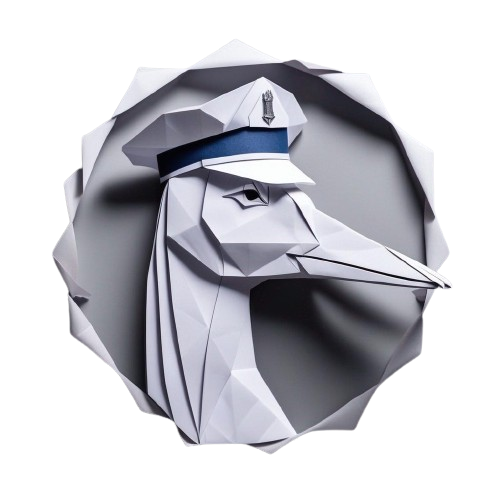
\includegraphics[height=0.8cm]{Gus}};
    \draw[->,ultra thick,red, decorate, decoration={random steps,segment length=3pt,amplitude=0.2pt}] (A) -- (B) node[midway, left] {$\distanceTwoTwoO m$};
    \draw[->,ultra thick,blue, decorate, decoration={random steps,segment length=3pt,amplitude=0.2pt}] (B) -- (C) node[midway, left] {$\distanceTwoTwoTw m$};
    
    \node [inner sep=0pt] at (Cp) {
\includegraphics[height=0.8cm]{DuckieGami}};
    \draw[->,ultra thick,blue, decorate, decoration={random steps,segment length=3pt,amplitude=0.2pt}] (Ap) -- (Bp) node[midway, left] {$\distanceTwoTwoTw m$};
    \draw[->,ultra thick,red, decorate, decoration={random steps,segment length=3pt,amplitude=0.2pt}] (Bp) -- (Cp) node[midway, left] {$\distanceTwoTwoO m$};
    
    \draw [decorate, 
	decoration = {calligraphic brace,mirror,
		raise=10pt,amplitude=5pt}] (Ap) -- (Cp) node[midway, right, xshift=0.5cm,line width=3pt] {$\distanceTwoTwoF m$};
\end{tikzpicture}}
%Distributivity
\subchapter{Distributivity}
{Duckie and Güs were starting to get frustrated. 
\paragraph{} "How are we going to get around this?" Güs asked.
\paragraph{} Duckie thought for a moment. He knew Güs could only compete for so long before becoming tired, and the more they flew, the better chance he would have. "How about a flying contest? We can do four parts instead of just three. Maybe then one of us will win."
\paragraph{} Gus agreed. His training from the goosepolice had given him excellent stamina, and was confident he could beat Duckie in long distance flying. 
\paragraph{} In the third contest, Güs traveled $\mathbf{2} km$, then $\mathbf{3} km$, and repeated that pattern $\mathbf{2}$ times. Duckie instead traveled $\mathbf{2} km$ $\mathbf{2}$ times, then $\mathbf{3} km$ $\mathbf{2}$ times. Did they tie?}
{Yes! Duckie flew $\mathbf{2}\ast(\mathbf{2} km + \mathbf{3} km)$, or $\mathbf{10} km$, and Güs flew $\mathbf{2}\ast\mathbf{2} km \ast \mathbf{3}\ast\mathbf{2} km$, or $\mathbf{10}km$.}
{Multiplying with an expression is the same as multiplying with each part of the expression. In other words: A$\ast$(B+C) = (A$\ast$B) + (A$\ast$C).}
{}
%Commutativity
\subchapter{Multiplicative Commutativity}
{At this point, Güs realized that Duckie was a very capable goose. When he first challenged Duckie, he expected winning to be a cakewalk, but Duckie ended up posing quite a challenge. Seeing Duckie's perseverance, Güs began to respect Duckie. He decided to give him another chance. He decided that the next contest should be a weightlifting competition, where whoever lifted the most amount of total weight would win. Duckie lifted $\mathbf{10} kg$  $\mathbf{3}$ times, whereas Güs lifted only $\mathbf{3} kg$ but did it $\mathbf{10}$ times. Did they tie?}
{Yes! Duckie lifted $\mathbf{10}kg\ast\mathbf{3}=\mathbf{30}kg$, and Duckie lifted $\mathbf{3}kg \ast \mathbf{10}=\mathbf{30}kg$. They lifted the same amount.}
{When multiplying, order does not matter. In other words: A$\ast$B = B$\ast$A.}
{\begin{tikzpicture} 
    \node [inner sep=0pt] at (0,15) {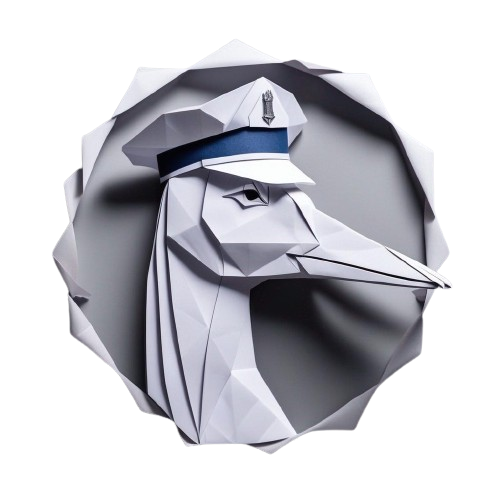
\includegraphics[height=0.8cm]{Gus}};
    \foreach \pos in {1,...,10} {	
        \MODULO{\pos}{2}{\rval}
        \SUBTRACT{\pos}{1}{\bl}
        \MODULO{\bl}{2}{\bval}
        \definecolor{col}{rgb}{\rval,0,\bval}
        \draw[->,ultra thick,col, decorate, decoration={random steps,segment length=3pt,amplitude=0.2pt}] (0,\pos *1.5 - 1.5) -- (0,\pos *1.5) node[midway, left] {$3 kg$};
    }
     \node [inner sep=0pt] at (1.5,15) {
\includegraphics[height=0.8cm]{DuckieGami}};
    \foreach \pos in {1,...,3} {	
        \MODULO{\pos}{2}{\rval}
        \SUBTRACT{\pos}{1}{\bl}
        \MODULO{\bl}{2}{\bval}
        \definecolor{col}{rgb}{\rval,0.7,\bval}
        \draw[->,ultra thick,col, decorate, decoration={random steps,segment length=3pt,amplitude=0.2pt}] (1.5,\pos *5 - 5) -- (1.5,\pos *5) node[midway, left] {$10 kg$};
    }
    
    \draw [decorate, decoration = {calligraphic brace,mirror, raise=10pt,amplitude=5pt}] (1.5,0) -- (1.5,15) node[midway, right, xshift=0.5cm,line width=3pt] {$30 kg$};
\end{tikzpicture}}
\paragraph{} Duckie and Güs landed on the forest floor, exhausted. They had realized that, no matter what the competition was, they were equally matched. They hadn't beat each other, but they \textit{had} won each other's respect. 
\paragraph{} "Why don't you join me?. You can make a difference!" asked Duckie.
\paragraph{} "I can't!" Güs cried. "What about my life in the goose police?"
\paragraph{} "Well, do you believe the golden goose is out there?"
\paragraph{} "Honestly, I'm not sure. Do you really think it will make the village a better place?"
\paragraph{} Duckie knew that there was the possibility the golden goose was a hoax, but knew the danger of disobeying the goose authorities, but knew he could help the entire village. 
\paragraph{} "You joined the goose police to help people", he reasoned. "You are clearly capable of making the dangerous journey, and if you can join me, you can do exactly that."
\paragraph{} Güs knew he was right. While he was afraid of what could happen along the journey, deep down, knew the tyranny of the authorities had gone too far. He decided to be brave and join Duckie. 
\paragraph{} "All right. I will join you!" he said resolutely. 
\chapter{Essential Algebra}
\paragraph{} Meanwhile, Duckie and Güs's various competitions made the goose authorities a bit confused. Because of Duckie and Güs's competitions, they lost track of where Duckie was. They decided that they needed to review their records of Duckie and Güs's locations, and try to figure out what they were doing on the fifth day. 
\vfill
\pagebreak
%Equality
\subchapter{Equality}
{Because Duckie and Güs were travelling together, they were always at the same position at any time.}
{Güs's position = Duckie's position. Duckie's distance from the village was $24km$, so Güs's position was also $24km$.}
{When two things are the same, we write this in mathematics as "=", or "equals".}
{\begin{tikzpicture}
    \coordinate (A) at (0,0);
    \coordinate (B) at (0,6.4);
    \coordinate (Ap) at (2,0);
    \coordinate (Bp) at (2,6.4);

    \node [inner sep=0pt] at (B) {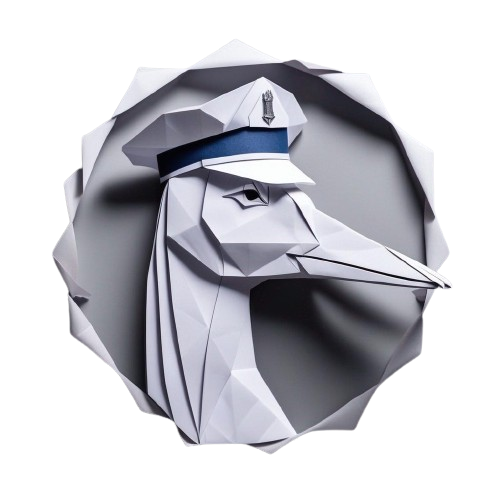
\includegraphics[height=0.8cm]{Gus}};
    \draw[->,ultra thick,red, decorate, decoration={random steps,segment length=3pt,amplitude=0.2pt}] (A) -- (B) node[midway, left] {$24 km$};
    \node [inner sep=0pt] at (Bp) {
\includegraphics[height=0.8cm]{DuckieGami}};
    \draw[->,ultra thick,blue, decorate, decoration={random steps,segment length=3pt,amplitude=0.2pt}] (Ap) -- (Bp) node[midway, left] {$24 km$};
\end{tikzpicture}
}
%The Equality Rule
\subchapter{The Equality Rule}
{The goose authorities, having trained Güs in the police academy, knew he was a very fast flyer. In fact, he had won the village racing competition for the past three years! Because Duckie and Güs were travelling together, they realized that every time Güs had flown ahead of Duckie, Duckie had to increase his position by the same amount to keep up.}
{Duckie's position + $\Delta$\footnote{$\Delta$ means "change in"}x = Güs's position + $\Delta$x.}
{What happens to one side of an equation must happen to the other side so that they are still equal.}
{\begin{tikzpicture}
    \coordinate (A) at (0,0);
    \coordinate (B) at (0,6.4);
    \coordinate (C) at (0,9.4);
    \coordinate (Ap) at (2,0);
    \coordinate (Bp) at (2,6.4);
    \coordinate (Cp) at (2,9.4);
    
    \node [inner sep=0pt] at (C) {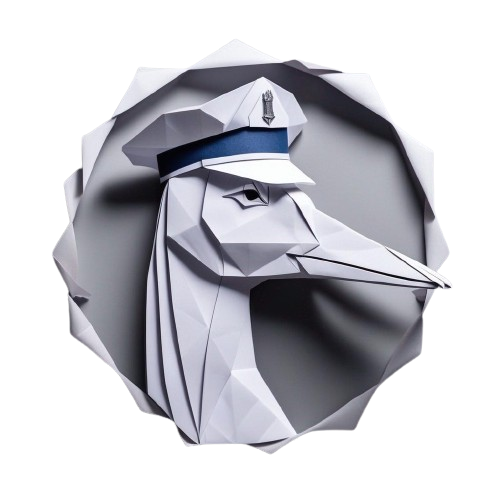
\includegraphics[height=0.8cm]{Gus}};
    \draw[->,ultra thick,red, decorate, decoration={random steps,segment length=3pt,amplitude=0.2pt}] (A) -- (B) node[midway, left] {$24 km$};
    \draw[->,ultra thick,orange, decorate, decoration={random steps,segment length=3pt,amplitude=0.2pt}] (B) -- (C) node[midway, left] {$16 km$};
    \node [inner sep=0pt] at (Cp) {
\includegraphics[height=0.8cm]{DuckieGami}};
    \draw[->,ultra thick,blue, decorate, decoration={random steps,segment length=3pt,amplitude=0.2pt}] (Ap) -- (Bp) node[midway, left] {$24 km$};
    \draw[->,ultra thick,orange, decorate, decoration={random steps,segment length=3pt,amplitude=0.2pt}] (Bp) -- (Cp) node[midway, left] {$16 km$};
    
    \draw [decorate, decoration = {calligraphic brace,mirror, raise=10pt,amplitude=5pt}] (Ap) -- (Cp) node[midway, right, xshift=0.5cm,line width=3pt] {$40 km$};
\end{tikzpicture}}
%Commutativity
\subchapter{Variables}
{The goose authorities were still a bit confused about Duckie and Güs's progress. They knew that there were $4$ competitions, and that they started at $24 km$. They also knew that they ended at $40 km$. How much did they travel on average in each competition?}
{\begin{center}$4x + 24 = 40 \linebreak 4x + 24 = 40 - 24 \linebreak 4x = 16 \linebreak \frac{4x}{4} = \frac{16}{4} \linebreak x = 4  $\end{center}}
{A letters or symbol can be used to represent a number which isn’t already known, such as "$x$". $4x + 16 = 40$ means that $4\ast(some number) + 16 = 40$.}
{\begin{tikzpicture}
    \coordinate (A) at (0,0);
    \coordinate (B) at (0,1);
    \coordinate (C) at (0,2);
    \coordinate (D) at (0,3);
    \coordinate (E) at (0,4);
    \coordinate (F) at (0,10);
    \coordinate (Ap) at (1.5,0);
    \coordinate (Bp) at (1.5,1);
    \coordinate (Cp) at (1.5,2);
    \coordinate (Dp) at (1.5,3);
    \coordinate (Ep) at (1.5,4);
    \coordinate (Fp) at (1.5,10);
    \coordinate (Af) at (3.4,0);
    \coordinate (Bf) at (3.4,1);
    \node [inner sep=0pt] at (F) {
\includegraphics[height=0.8cm]{DuckieGami}};
    \draw[->,ultra thick,blue, decorate, decoration={random steps,segment length=3pt,amplitude=0.2pt}] (A) -- (B) node[midway, left] {$? km$};
    \draw[->,ultra thick,blue, decorate, decoration={random steps,segment length=3pt,amplitude=0.2pt}] (B) -- (C) node[midway, left] {$? km$};
    \draw[->,ultra thick,blue, decorate, decoration={random steps,segment length=3pt,amplitude=0.2pt}] (C) -- (D) node[midway, left] {$? km$};
    \draw[->,ultra thick,blue, decorate, decoration={random steps,segment length=3pt,amplitude=0.2pt}] (D) -- (E) node[midway, left] {$? km$};
    \draw[->,ultra thick,green, decorate, decoration={random steps,segment length=3pt,amplitude=0.2pt}] (E) -- (F) node[midway, left] {$24 km$};
    \draw [decorate, decoration = {calligraphic brace, raise=35pt,amplitude=5pt}] (A) -- (F) node[midway, left, xshift=-1.5cm,line width=3pt] {$40 km$};
    
    \draw[->,ultra thick,blue, decorate, decoration={random steps,segment length=3pt,amplitude=0.2pt}] (Ap) -- (Bp) node[midway, left] {$? km$};
    \draw[->,ultra thick,blue, decorate, decoration={random steps,segment length=3pt,amplitude=0.2pt}] (Bp) -- (Cp) node[midway, left] {$? km$};
    \draw[->,ultra thick,blue, decorate, decoration={random steps,segment length=3pt,amplitude=0.2pt}] (Cp) -- (Dp) node[midway, left] {$? km$};
    \draw[->,ultra thick,blue, decorate, decoration={random steps,segment length=3pt,amplitude=0.2pt}] (Dp) -- (Ep) node[midway, left] {$? km$};
    \draw[->,ultra thick,red, decorate, decoration={random steps,segment length=3pt,amplitude=0.2pt}] (Fp) -- (Ep) node[midway, left] {$-24 km$};
    \draw [decorate, decoration = {calligraphic brace,mirror, raise=10pt,amplitude=5pt}] (Ap) -- (Ep) node[midway, right, xshift=0.5cm,line width=3pt] {$16 km$};
    
    \draw[->,ultra thick,blue, decorate, decoration={random steps,segment length=3pt,amplitude=0.2pt}] (Af) -- (Bf) node[midway, left] {$4 km$};
\end{tikzpicture}}.
\chapter{Ratios and Fractions}
\paragraph{} It took a lot of work, but the authorities finally figured out where Duckie was. They noticed that Duckie and Güs made quite a bit of progress, which was very bad news for them. They wanted to use this information to try to stop them. Because of Güs defecting to join Duckie's journey, they realized that sending other policegeese would make it hard to keep their power in the village. 
\paragraph{} Through their past migrations, they knew lots of bounty hunters along the way, and they believed that they could have them set traps. These bounty hunters were famously clever, and each of them decided to use specific strategies to help them catch Duckie and Güs.
\vfill
\pagebreak
%Ratios
\subchapter{Ratios}
{The first bounty hunter decided to look at the entire journey, and set up traps every P4 km. He estimated that the entire journey was R km long. Duckie having guessed this fairly obvious scheme,  thought that if he knew how many traps there would be, he could avoid them. For every km in the entire journey, there would be a trap every P4 km. How many traps will there be on the journey?}
{For every P4 km Duckie has to travel out of (R) km overall, there will be a trap. That means that there is a trap every $\frac{R}{P4}$ km of the journey. For every one km in P4, there are S km in the journey (R), which means that there are S lengths of size P4 within R. There are $\frac{S}{1}$, or S traps.}
{A ratio is a certain amount for each of another amount, and is written as $\frac{A}{B}$. Break up A into B equal parts.}
{}
%Multiplying with Fractions
\subchapter{Multiplying with Fractions}
{Using this knowledge, Duckie figured out how to avoid the first bounty hunter's traps. The second bounty hunter decided to prepare better than the first hunter. He realized that km are a very large unit for geese, so decided to start measuring the distance Duckie and Güs flew in a unit he created called "goosemeters" (gm). This meant that he needed to change their position from kilometers into goosemeters. There are U gm for every V m. To help beat the second bounty hunter, Duckie and Güs decide to also measure using gms. How many gms are in P4 km?}{
$\frac{Ugm}{Vm}*\frac{Rm}{1}*\frac{1}{S}=\frac{UR}{VS} gm$.
}{Like any number, multiplying by a ratio represents scaling by a certain amount. Imagine a rubber band which is P long, which you can stretch and squish. Multiplication represents scaling the band such that $P*\frac{A}{B}$ is the new length of the band. This is the same as $\frac{P*A}{B}$, or $\frac{P}{B}*A$. This can be seen as dividing the band into B equal parts, then taking one of those parts A times. \paragraph{} Notice that that $\frac{A}{B}$ can create numbers in between 0, 1, 2, etc.}{MultiplyingFractions.png}
%Comparing Fractions
\subchapter{Comparing Fractions}
{Duckie thought that if he traveled enough in one day, the bounty hunter would become confused and leave them alone. On the eighth day, Duckie and Güs traveled an additional W/X of the journey. If Duckie traveled more on the eighth day than the combined previous 7 days, the bounty hunter would become confused and stop chasing Duckie. Has Duckie managed to confuse the bounty hunter?}{Duckie realizes that \begin{center}
    $\frac{X}{X}=1$ \linebreak
    $\frac{UR}{VS}$ * 1 = $\frac{UR}{VS}$ \linebreak
    $\frac{UR}{VS}$ * $\frac{X}{X}$ = $\frac{UR}{VS}$ = $\frac{URX}{VSX}$\linebreak  Which means $\frac{UR}{VS}$  is same as  $\frac{URX}{VSX}$ \linebreak\linebreak
    \textit{similarly}
    $\frac{W}{X}$ =$\frac{WVS}{VSX}$
\end{center}
\paragraph{} Now, we can compare the equal size parts together. $\frac{WVS}{VSX} < \frac{URX}{VSX}$}{We can only deal with fractions together using same-size parts. We can chop up one fraction by multiplying it by another fraction equal to one. If the \textit{denominator}s (the bottom number of the fractions) are the same, the fractions have same sized parts.}{ComparingFractions}
%Adding Fractions
\subchapter{Adding Fractions}
{Despite Duckie's best efforts, he was unfortunately not able to confuse the bounty hunter. He was starting to get worried, but Güs had a genius idea. If they could find out where they were along the journey, they might have been able find a new route, which would take them away from the hunter's grasp! They traveled $\frac{WVS}{VSX}$, then they traveled $\frac{URX}{VSX}$. How much of the journey have Duckie and Güs traveled?}{Duckie and Güs have traveled
$\frac{WVS}{VSX}+\frac{URX}{VSX}\linebreak=\frac{WVS+URX}{VSX}\linebreak=\frac{WVS+URX}{VSX}$ths of the journey.}{When adding fractions, break up each fraction so that they are in terms of same-size parts (or having a common denominator). Then, add the numerators as usual.}{AddingFractions}
\paragraph{} Duckie and Güs sighed in relief. After running for bounty hunters for two days and two nights, they were exhausted. They decided to travel slower for a few days and enjoy the scenery. 
\paragraph{} "I can't believe how persistent the goose authorities are." Duckie sighed. "I knew this journey would be tough, but I wasn't expecting bounty hunters!"
\paragraph{} Güs considered this. He had worked with the goose authorities, and knew their patterns. He realized how unusual this was. "I agree, the authorities must really be desparate".
\paragraph{} Just as Duckie opened his beak to reply, he felt a sudden weight on his shoulders, and began spiraling out of control. It was a net! Another bounty hunter must have set a trap! He started falling down fast, gaining speed as he went. \textbf{Crash!}. Duckie fell to the ground with a thud. Güs hurriedly landed next to him. 
\paragraph{} "Are you alright Duckie‽" he cried in alarm.
\paragraph{} "I'm all right, but I think I need to rest my wing for a few days", Duckie winced. He felt that he hadn't broken a wing, but saw some bruising, and knew he would need time to heal. 
 \paragraph{} "The forest is dangerous though! We can't stay here in the open with all the predators!"
 \paragraph{} "I think my friend Bessie the cow's farm is close enough to walk to from here," Duckie said. "I think she will be able to help keep us safe from the goose authorities."
 \paragraph{} Together, they waddled to Bessie's farm.
 \chapter{Rectangles, Perimeter, and Area}
 \paragraph{} After walking all afternoon, Duckie and Güs finally arrived at Bessie's farm. Despite the bad luck with the net, it was a beautiful afternoon, and the pair couldn't help but feel a sense of calm as the walked up to Bessie's barn.
 \paragraph{} Bessie was sitting outside, chewing on some grass.
 \paragraph{} "Hey there Duckie! How's it going? Who's your friend there?" she moo'd.
 \paragraph{} "Hi Bessie", Duckie greeted. "This is my friend Güs. We are looking for the golden goose of legend, but I need some help."
 \paragraph{} "Of course! What do you need?" asked Bessie.
 \paragraph{} "I hurt my wing, and I need to rest here for a few days. The goose authorities sent some bounty hunters after me, and I need you to keep me safe from them," Duckie asked hesitantly.
 \paragraph{} "Wow, that sounds serious. Feel free to stay as long as you like" Bessie turned around to look at Güs. "While Duckie's is getting better, I could use some help on the farm. It's grass-planting season, and it would be much appreciated if you could help me out on the farm."
 \paragraph{} Güs, enthusiastically agreed. "That sounds great!"
 \pagebreak
%Area of Rectangles
 \subchapter{Area of Rectangles}
{On the ninth day of the journey, Güs began working on the farm. His first task was to fly around and scatter grass seeds on the farm. As he went into the store room to find the bags of seeds, he realized he needed to know how many bags of seeds he needs to bring with him. Bessie told him that each bag of seeds can cover a square of grass that is 1 m wide and 1 m across. Güs also knows that the farm is $300 m$ high and $400 m$ wide. How many bags of seeds does Güs need to carry?}
{There are 300 rows of grass, where each row is made of 400 1 by 1 squares. This means that there are $300\ast 400 = 300\ast 400 meters^{2}$ of grass, and that Güs needs to carry $300\ast 400$ bags.}
{Area is how much space an object takes up. When measuring a 2d shape, we find how many 1 by 1 squares the object fills. When measuring the area of a 3d shape, we find how many 1 by 1 by 1 cubes the object fills. Multiplying the length of each side together for "square" shapes gives us the area. (We will discuss area further with integrals).}
{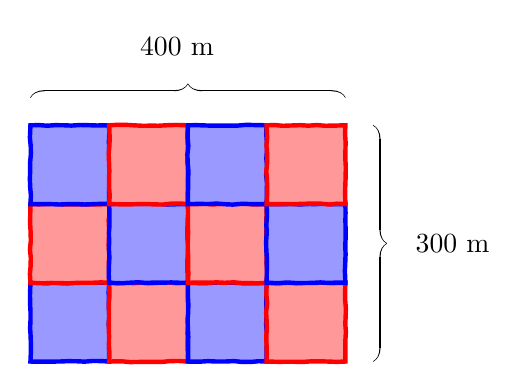
\begin{tikzpicture}
    \coordinate (A) at (0,0);
    \coordinate (B) at (0,3);
    \coordinate (C) at (4,3);
    \coordinate (D) at (4,0);
    
    \foreach \xpos in {1,...,4} {	
        \foreach \ypos in {1,...,3} {
            \SUBTRACT{\xpos}{1}{\llxpos}
            \SUBTRACT{\ypos}{1}{\llypos}
            \ADD{\llxpos}{\llypos}{\s}
            \MODULO{\s}{2}{\redval}
            \ADD{\s}{1}{\b}
            \MODULO{\b}{2}{\blueval}
            \definecolor{col}{rgb}{\redval,0,\blueval}
            \filldraw[fill=col!40!white, draw=col, ultra thick, decorate, decoration={random steps,segment length=3pt,amplitude=0.2pt}] (\llxpos,\llypos) rectangle (\xpos,\ypos);
        }
    }
    
    \draw [decorate, decoration = {calligraphic brace, raise=10pt,amplitude=5pt}] (C) -- (D) node[midway, left, xshift=2cm,line width=3pt] {300 m};
    \draw [decorate, decoration = {calligraphic brace, raise=10pt,amplitude=5pt}] (B) -- (C) node[midway, left, xshift=0.5cm, yshift=1cm,line width=3pt] {400 m};
\end{tikzpicture}}
%Area of Square Edge Triangles
\subchapter{Area of Square Edge Triangles}
{As Güs took off, he noticed that the farm was split into two equal parts along the diagonal to make space for Bessie's pet human Farmer John. He realized that here, he could not plant grass, as Farmer John needed it for corn. How many bags of grass should Güs plant?}
{The farm is divided in half, so Güs only needs to plant half of his bags. $\frac{1}{2}\ast 300m\ast 400m\linebreak=1200m^{2}\ast\frac{1}{2} \linebreak=600m^{2}$.}
{Right triangles (triangles with a square edge), are rectangles that have been split in half along the diagonal. This means that the area of a right triangle with side lengths x and y has an area of $\frac{x\ast y}{2}$.}
{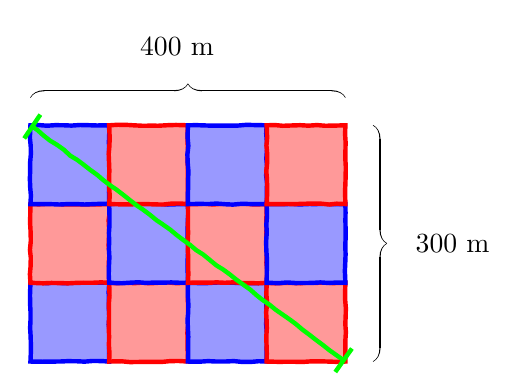
\begin{tikzpicture}
    \coordinate (A) at (0,0);
    \coordinate (B) at (0,3);
    \coordinate (C) at (4,3);
    \coordinate (D) at (4,0);
    
    \foreach \xpos in {1,...,4} {	
        \foreach \ypos in {1,...,3} {
            \SUBTRACT{\xpos}{1}{\llxpos}
            \SUBTRACT{\ypos}{1}{\llypos}
            \ADD{\llxpos}{\llypos}{\s}
            \MODULO{\s}{2}{\redval}
            \ADD{\s}{1}{\b}
            \MODULO{\b}{2}{\blueval}
            \definecolor{col}{rgb}{\redval,0,\blueval}
            \filldraw[fill=col!40!white, draw=col, ultra thick, decorate, decoration={random steps,segment length=3pt,amplitude=0.2pt}] (\llxpos,\llypos) rectangle (\xpos,\ypos);
        }
    }
    
    \draw[|-|,ultra thick,green, decorate, decoration={random steps,segment length=3pt,amplitude=0.2pt}] (B) -- (D) node[midway, left] {};
    
    \draw [decorate, decoration = {calligraphic brace, raise=10pt,amplitude=5pt}] (C) -- (D) node[midway, left, xshift=2cm,line width=3pt] {300 m};
    \draw [decorate, decoration = {calligraphic brace, raise=10pt,amplitude=5pt}] (B) -- (C) node[midway, left, xshift=0.5cm, yshift=1cm,line width=3pt] {400 m};
\end{tikzpicture}}
\subchapter{Pythagorean Theorem}
{Güs started planting grass. He remembered from school that grass spread rapidly, and so decided that to keep Farmer John's corn safe, he would make a small fence along the diagonal. How long of a fence does Güs need to buy?}
{$300m\ast 300m + 400m\ast 400m = 500m\ast 500m$. Güs needs to buy $500m$ of fence.}
{In a right triangle, the lengths of sides are related to one another. In such a triangle, a$\ast$a + b$\ast$b = c$\ast$c, where c is the diagonal length in the triangle. This relationship is called the \textit{pythagorean theorem}. \footnote{A proof of the theorem is found here: \url{https://www.mathsisfun.com/geometry/pythagorean-theorem-proof.html}}}
{\tikzset{square/.style={minimum size=#1,draw},
measureme/.style={execute at begin to={
\path let \p1=($ (\tikztostart) - (\tikztotarget) $),\n1={veclen(\x1,\y1)}
in \pgfextra{\xdef#1{\n1}};}}}
\begin{tikzpicture}
\filldraw[measureme=\mylen](0,0) 
to node[midway,sloped,above,square=\mylen,fill=blue!20,draw=blue, ultra thick]{\xdef\mylenC{\mylen}} node[midway,left=3pt]{$C$} (1,2)
to node[midway,sloped,above,square=\mylen,fill=red!20,draw=red, ultra thick]{\xdef\mylenB{\mylen}} node[midway,right=3pt]{$B$} (1,0) 
to node[midway,sloped,below,square=\mylen,fill=purple!20,draw=purple, ultra thick]{\xdef\mylenA{\mylen}} node[midway,below=3pt]{$A$} (0,0);
\begin{scope}[yshift=-5cm]
 \node[square=\mylenB,fill=red!20!white,draw=red,ultra thick](B) {$BxB$};
 \node[left=2pt of B] (plus) {$+$};
 \node[left=2pt of plus,square=\mylenA,fill=purple!20!white,draw=purple, ultra thick](A) {$AxA$};
 \node[right=2pt of B] (eq) {$=$};
 \node[right=2pt of eq,square=\mylenC,fill=blue!20!white,draw=blue, ultra thick](C) {$CxC$};
\end{scope}
\end{tikzpicture}}
%Perimeter
\subchapter{Perimeter of a Shape}
{After Güs finished planting grass, he decided to take a break for lunch. \paragraph{} "Aaaah," he sighed, contented. As he looked out at the farm, he noticed a discontented look on Bessie's face. \paragraph{}"What's the issue?" he asked. \paragraph{} "It's this fence." Bessie replied. "It's falling apart and we have to look at it all day." Güs decided that to thank her for letting them stay for the night, he would buy her a new fence. How many meters of fence does Güs need to buy?}
{Two sides of the fence are $300 m$ long, and two sides of the fence are $400 m$ long. That means that there are $300 m + 300 m + 400 m + 400 m = 2\ast 300 m+ 2\ast 400 = 2\ast(300 m + 400m) = 2\ast 700 = 1400 m$ of fence.}
{Surface, or perimeter, is the size of the edge of an object. When measuring a 2d shape, we find how many lines of length 1 can fit around the object. When measuring a 3d shape, we find how many 1 by 1 squares fit around the object. (We will discuss this further with integrals).
The perimeter is the sum of all of the side lengths. Because 2 of the side length of the sides of a rectangle are always the same, 2x+2y is its perimeter, which can also be written as 2(x+y).}
{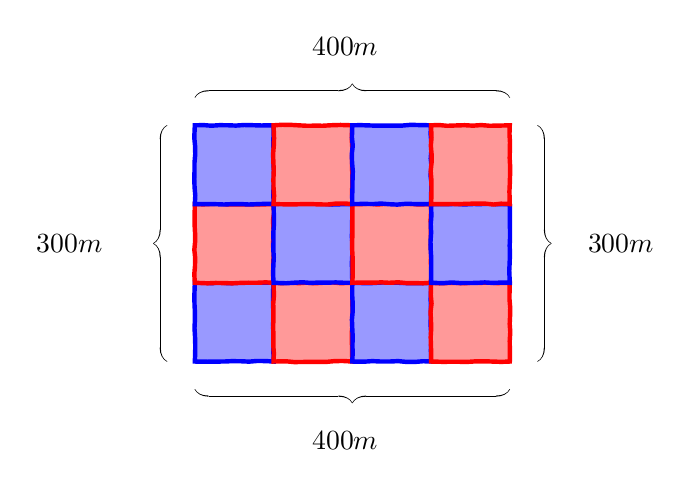
\begin{tikzpicture}
    \coordinate (A) at (0,0);
    \coordinate (B) at (0,3);
    \coordinate (C) at (4,3);
    \coordinate (D) at (4,0);
    
    \foreach \xpos in {1,...,4} {	
        \foreach \ypos in {1,...,3} {
            \SUBTRACT{\xpos}{1}{\llxpos}
            \SUBTRACT{\ypos}{1}{\llypos}
            \ADD{\llxpos}{\llypos}{\s}
            \MODULO{\s}{2}{\redval}
            \ADD{\s}{1}{\b}
            \MODULO{\b}{2}{\blueval}
            \definecolor{col}{rgb}{\redval,0,\blueval}
            \filldraw[fill=col!40!white, draw=col, ultra thick, decorate, decoration={random steps,segment length=3pt,amplitude=0.2pt}] (\llxpos,\llypos) rectangle (\xpos,\ypos);
        }
    }
    
    \draw [decorate, decoration = {calligraphic brace, raise=10pt,amplitude=5pt}] (C) -- (D) node[midway, left, xshift=2cm,line width=3pt] {$300 m$};
    \draw [decorate, decoration = {calligraphic brace, raise=10pt,amplitude=5pt}] (B) -- (C) node[midway, left, xshift=0.5cm, yshift=1cm,line width=3pt] {$400 m$};
    \draw [decorate, decoration = {calligraphic brace, raise=10pt,amplitude=5pt}] (A) -- (B) node[midway, left, xshift=-1cm,line width=3pt] {$300 m$};
    \draw [decorate, decoration = {calligraphic brace, raise=10pt,amplitude=5pt}] (D) -- (A) node[midway, left, xshift=0.5cm, yshift=-1cm,line width=3pt] {$400 m$};
\end{tikzpicture}}
\section{Shoelace Theorem}
\paragraph{} The shoelace formula is a tool which lets us find the area of any polygon. Go around the vertex's of the polygon, where the current vertex's coordinates are $x_i, y_i$ and the next vertex's coordinates are $x_{i+1}, y_{i+1}$ \linebreak
$A:={\frac{1}{2}}\sum_{cyc} (x_iy_{i+1}-x_{i+1}y_i)$.
\chapter{Circles and Angles}
\paragraph{} On the 10th day, Bessie had an issue: Farmer John was bored and kept causing trouble on the farm. Rather than letting her and the other cows graze, he was trying to cut down their grass. To keep him entertained and away from the grass, Bessie decided to create crop circles in the corn field.
\paragraph{} "Duckie!" she called. "Want to help make some crop circles?"
\paragraph{} "Sure! I think it will be great for helping my wing recover!" Duckie replied.
\vfill
\pagebreak
 \subchapter{Angles}
 {Bessie and Duckie came up with a plan to draw their circles. They decided that Duckie would fly around Bessie, staying exactly Q m away from Bessie at each point. To make sure Duckie is exactly the same distance, Bessie would spin around and look at him at any given point. Bessie knows she will get dizzy if she spins too much, so decides to keep track of how much she has turned at any moment.}
 {}
 {The number of meters between the Duckie and Bessie is called r, or the “radius”. When Duckie has flown r meters around Bessie, the amount Bessie has turned is a “radian”.}
 {Addition}
 \subchapter{Drawing a single Circle}
 {Bessie and Duckie began to draw the first circle, but ran into an issue. She didn't know when to stop spinning! How many radians does Bessie have to turn so that Duckie makes a full circle (and she looks in the same place she started)?}
 {}
 {When Duckie has flown a full circle around Bessie and Bessie was looking in the same direction where she started, she had turned around 2$\pi$ radians. This amount Bessie turned cannot be written as a fraction, and so is called “irrational”. This specific irrational number has the name “pi”. 
 \paragraph{} For convenience, approximate $\pi$ to be $\frac{22}{7}$ (the actual value of pi is slightly smaller).}
 {Addition}
  \subchapter{Perimeter of a Circle}
 {After some effort calculating, Duckie drew one full circle around Bessie. But, because of his injured wing, he began to feel a bit tired. He decided that in the full day, he would only fly W m so that his wing would recover properly. How much has Duckie flown?}
 {For every radian Bessie turned, Duckie flew R m. Because Bessie turned 2$\pi$ radians, Duckie must have turned $2\pi Q$ m.}
 {The perimeter of a circle is always $2\pi r$, where r is radius of the circle.}
 {Addition}
 \subchapter{Trigonometric Functions}
 {After resting for a few minutes, Duckie and Bessie started drawing their next circle. They decided that, to help give Farmer John some contrast, they would make it have a radius of 1. While creating the circle, tragedy struck! Duckie lost track of where he was! He sees that Bessie turned $\frac{\pi}{4}$ radians. What is Duckie's vertical position? What is Duckie's horizontal position?}
 {}
 {Take a line of length 1. As we rotate the line, we can see it has both a height and a width. When it starts, it has width but not height. When it rotates $\frac{\pi}{2}$ radians it has height but not width. When x is the angle rotated, the width at each angle (or the adjacent side/the diagonal side) is cos(x). The height at each angle (or the opposite side/the diagonal side) is sin(x).}
 {Addition}
  \subchapter{Trigonometric Identities}
 {Duckie, tired, but with a healed wing, sat down. He and Bessie were ready to take the day off, and he was ready to start flying the next day. Güs, who had been planting grass, walked over to them. 
 \paragraph{} "Hey Guys! How was your work in the cornfield?"
 \paragraph{} "It was pretty good!" Bessie replied. "We were drawing circles for Farmer John while you planted grass."
 \paragraph{} Güs looked at Bessie in surprise. "That's what you were doing? I thought you were tracing the point of an arrow where the width\texttimes the width plus the height\texttimes the height equaled one!"
 The trio looked at each other in confusion. Who is right?}
 {They were all right! The width of the arrow is cos(x), and the height of the arrow is sin(x). Through pythagorean theorem, the length of the arrow must be 1, which is also the radius that Duckie flew.}
 {sin(x) * sin(x) + cos(x) * cos(x) = 1*1 = 1.}
 {Addition}
\chapter{Sets and Functions}
\paragraph{} It was time for Duckie and G{\"u}s to continue on their journey. They had enjoyed spending time with Bessie, but they still needed to get to the Golden Goose.
\paragraph{} "What are we going to do about the Bounty Hunters?" G{\"u}s asked Duckie nervously. They both were concerned about the bounty hunters' traps.
\paragraph{} "I'm not sure" Duckie replied, "But we will have to keep moving. Hopefully we find something or someone along the way who can help".
\paragraph{} As the duo began to fly once more that evening, they saw an approaching flock of geese behind them.
\paragraph{} "Quick! Land!" Duckie cried. In a flash, in a rustle of feathers, the pair landed and waited, hoping to go unnoticed.
\paragraph{} There was the squaking of the the voices of the other group of geese as they landed beside Duckie and G{\"u}s.
\paragraph{} "Hi, how's it going?" one of the geese asked. This surprised Duckie. He was expecting to be taken away to the goose village, but he wasn't expecting a greeting.
\paragraph{} "Hello..." Duckie said cautiously. "Who are you? Have the goose authorities sent you?"
\paragraph{} "We are just a gaggle from the north. My name is Snow. What are the goose authoriies?". Duckie relaxed. Clearly, these geese wouldn't take them away. G{\"u}s, having had experience from journeying with the Goose Police, knew the value of traveling with a group.
\paragraph{} "Oh, I guess if you don't know who they are, they aren't that important to you," G{\"u}s said to Snow. "We are trying to find the golden goose, and it seems like you are heading in the same direction as us. Mind if we join you?"
\paragraph{} "Alright!" Snow said. "But you'll have to join our dance!".
\vfill
\pagebreak
\subchapter{Cartesian Product}
{That night, the new flock decided to have their traditional nightly dance. It was a partners dance, with the following rules: geese with red feet were one group, and the geese with blue feet were another group. Each of the red geese partnered with each of the blue geese, where a red goose lead. The group of red geese in the dance was \{G{\"u}s, Snow, Grey, Blue\}. The group of blue geese was \{Duckie, Barnie, Swan\}. How many ways could the geese have formed pairs? What are those pairs?}
{All the pairs that the Geese could have formed were \{(G{\"u}s, Duckie), (G{\"u}s, Barnie), (G{\"u}s, Swan), (Snow, Duckie), (Snow, Barnie), (Snow, Swan), (Grey, Duckie), (Grey, Barnie), (Grey, Swan), (Blue, Duckie), (Blue, Barnie), (Blue, Swan)\}. There were 4 geese with red feet, and 3 geese with blue feet. There were \opmul{4}{3} ways to form pairs}
{A set is an unordered collection of things. If there are two sets, $A$ and $B$, the cartesian product ($AxB$) are the pairs $(a, b)$ where $a\in$ \footnote{$\in$, means "is in the set"} $A$ and $b\in B$.}
{}
\subchapter{Relations}
{Maggie, one of the blue footed geese and, the organizer of the dance, looked over G{\"u}s's shoulder to see what he was doing. \paragraph{} "Hi there! Whatcha doin'?" she asked inquisitively.
\paragraph{} "Nothing much, I'm just trying to figure out how the dance works. Can you take a look?"
\paragraph{} "Of course!" Maggie considered his drawings. "It seems like you are on the right track, but I think Snow and Barnie like to dance different styles. Maybe they shouldn't be a possible pair?"
\paragraph{} G{\"u}s removed their pairing from his plans. "So all of the pairs in the new set are in the original set."
\paragraph{} How many sets of pairs could Maggie and G{\"u}s make out of the original cartesian product?}
{Maggie and G{\"u}s can quite a few sets. These include \{\}, the $AxB$ itself, all sets with only a single pair, all the sets with only two pairs, etc.}
{If a set $A$ (also called the domain) is a subset of set $B$ (also called the codomain), then every element in set $A$ is also in set $B$. For every set $A$, there are $2^{|A|}$ possible subsets which can be made $\footnote{|A| means size of A}$. A subset of a cartesian product called is a relation.}
{}
\subchapter{Functions}
{G{\"u}s and Maggie continued to plan, and decided to come up with the list of pairs of geese. 
\paragraph{} "Hmm..." Maggie thought, looking at the list of relations. "There are not enough blue geese for each goose to have their own partner. How can we make sure each goose has their own partner?"
\paragraph{} G{\"u}s thought for a moment. "Maybe some of the blue geese can take turns switching between partners?"
\paragraph{} "I'm not sure, but maybe it would work. Let's try it out!"
Come up with a possible set of pairs dance partners Maggie and G{\"u}s could have formed.}
{Maggie and G{\"u}s eventually decided on the following set of dance partners \{(G{\"u}s, Barnie), (Snow, Barnie), (Grey, Swan), (Blue, Duckie)\} with Maggie sitting aside}
{A function is a special type of relation between the sets $A$ and $B$. In a function, in every pair $(a, b)$ (where $a\in A$ and $b\in B$), $a$ only maps to a single output. This allows us to say that the $f(a) = b$, or that the value $a$ maps to the value $b$.}
{}
\subchapter{Types of Functions}
{As the dance began, Maggie watched the other geese dance. G{\"u}s noticed her watching, and came over. 
\paragraph{} "Why don't you come over and dance with us?" G{\"u}s asked. 
\paragraph{} "Ah, you don't want me to dance, I don't to mess up the fun. Besides, this way, the blue geese don't have to worry about switching partners."
\paragraph{} G{\"u}s looked over. "Don't worry about that, it's fun! Besides, now there aren't enough red geese. C'mon!".
\paragraph{} Maggie hesitated, "Well, let's see how they do on their own for now."
\paragraph{} "You'll do great!"
\paragraph{} "Alright! Let's dance!" 
\paragraph{} G{\"u}s and Maggie went back to the dance floor together. 
What does the new function mapping red geese with blue geese look like?}
{With all the geese dancing, the red geese and new geese were mapped so that the dancing partners were \{(G{\"u}s, Maggie), (Snow, Barnie), (Grey, Swan), (Blue, Duckie)\}}
{A function where every element in the domain has a different mapping is called "one-to-one". A function where every element in the codomain is mapped to is called "onto". A function which is both one-to-one and onto is called "bijective".}
{}
\subchapter{Inverse of Functions}
{As the first dance came to a close, Maggie went to the makeshift stage to begin the next dance.  
\paragraph{} "All right everyone!" she announced happily. "Same dance, but this time, blue geese lead!" 
\paragraph{} The geese cheered, and began the dance again with the blue geese taking the lead. Was this new pairing a function? If so, what did it look like?}
{The new pairing was \{(Maggie, G{\"u}s), (Barnie, Snow), (Swan, Grey), (Duckie, Blue)\}. This new pairing was also a function, because every first element only mapped to a single output. For example, originally, $f($G{\"u}s$)= $Maggie, but now $f^{-1}($Maggie$) = $G{\"u}s}
{The inverse of a function $f(x)$ is written as $f^{-1}(x)$. The input of of $f$ is the output of $f^{-1}$, and the output of $f$ is $f^{-1}$. In other words, if $f(a)=b$, then $f^{-1}(b) = a$. In order for there to be an inverse function for $f(x)$, $f(x)$ must be bijective. }
{}
\subchapter{Continuous Functions}
{As G{\"u}s and Maggie danced with each other, they realized that they could also explain the movement of the dance as a function. $f(t) = -t\ast t+10$, where $t$ was the number of minutes since the dance began, and $f(t)$ represented how far they stood from the stage. What was G{\"u}s and Maggie's position when they had danced for 3 minutes?}
{$f(3) = -3\ast 3 + 10$\linebreak $f(3)=1$.\linebreak When they had danced for three minutes, G{\"u}s and Maggie were standing 1 meter from the stage.}
{Functions can be written as pair explicitly, or with a formula. When making a function using a formula, the pairs are $(x, f(x))$}
{}

\chapter{Polynomials}
\paragraph{} The next morning, Duckie and G{\"u}s looked out of their campground. 
\paragraph{} "Looks like we are almost there. I've been talking to Maggie and I think she wants to come with us to find the Golden Goose" G{\"u}s remarked.
\paragraph{} "That's great!" Duckie said. "We shouldn't count our geese before they hatch though. Even though we are almost there, we are going to start the most difficult part of the journey. Look at the mountain!"
\paragraph{} The looked at the mountain and saw it towering above them. 
\paragraph{} "I agree. I think we need to prepare."
\paragraph{} As the rest of the geese woke up, Duckie and G{\"u}s stood up and announced their departure. 
\paragraph{} "Hello everyone. Thank you for your hospitality. I want to make sure we can get there quickly so that we can save our village, so we need to travel fast. We need to continue on our journey. Would anyone like to come with us?"
\paragraph{} Maggie stepped forward. "I'll join!"
\paragraph{} "Great!" Duckie said. 
\vfill
\pagebreak
\subchapter{Polynomial Functions}
{\paragraph{} Duckie, Maggie, and G{\"u}s began flying towards the mountain. 
\paragraph{} "Wow thats pretty steep. We should probably try to figure out where it is and what it looks like." Maggie noted. 
\paragraph{} "That makes sense" Duckie said. "Looking at the mountain, it looks to me like it touches the ground at two points. But how will we figure out how the mountain looks?"
\paragraph{} Maggie pondered this over this for a moment.
\paragraph{} "What if we made a function? It can map every position on the ground to the height of the mountain at that point. Since it touches the ground at two points, h(x) = 0"
\paragraph{} "That's a good idea" Gus said. "But where does it touch the ground? Maybe we can say it touches the ground when $x_1$ = ? and $x_2$ = ?"
\paragraph{} What is h(x)?}
{
	\paragraph{} We can separate the function into two parts. We want the function to be 0 when x is 0. 
	$x-x_1$ will be 0 when $x = x_1$. Similarly, $x-x_2$ will be 0 when $x=x_2$. 
	\paragraph{} $0\ast$any number is 0. 
	\paragraph{} Because of this, we can set $h(x)=(x-x_1)(x-x_2)$.
}
{A polynomial function is a function where f(x) is the sum of terms, such that each term is a constant multiplied with x raised to a natural number. In other words, $\sum a*x^{k}$ s.t. $a \in \mathbb{R}, k \in \mathbb{N}$.}
{}

\subchapter{Polynomial Functions}
{\paragraph{} Duckie thought for a moment. 
\paragraph{} "I am not so sure about that actually. To me, the function looks like $ax^2-bx+c$"
\paragraph{} Maggie was hesitant "Won't this give us the incorrect ground locations?" 
\paragraph{} "I'm not sure. How can we make sure?"
\paragraph{} Where would the mountain touch the ground if $h(x)=ax^2-bx+c$?
}
{\paragraph{} $\frac{-b \pm \sqrt{b^2-4ac}}{2a} = $
\paragraph{} $\frac{-b \pm \sqrt{b^2-4ac}}{2a} = $
\paragraph{} $\frac{-b \pm \sqrt{b^2-4ac}}{2a} = $}
{The roots of a polynomial with degree two are $\frac{-b \pm \sqrt{b^2-4ac}}{2a}$}
{}

\subchapter{Polynomial Functions}
{ The trio sped up as they approached the mountain. As they approached, it seemed to grow taller and taller and wider and wider. 
	They could see the snowcapped peaks clearly, and realized they had made the mistake. 
	The mountain was x meters taller than they had originally thought. 
	\paragraph{} "What can we do?" Gus pondered aloud.
	\paragraph{} "Can we modify the function we made before?" Maggie asked.
	\paragraph{} Modify the height of the function so that every point is x points higher and y points to the right.
}
{
	$h(x) = h(x) + x$
}
{ A function can be transformed in 3 ways.
	\begin{enumerate}
		\item It can be shifted up and down by adding a constant from the overall function
		\item It can be shifted to the left and right by subtracting a constant from x
		\item It can be compressed by multiplying x by a constant.
	\end{enumerate}
}
{}

What is an exponent?\linebreak
They have not seen the top of the mountain yet, so they assume that it is a quadratic function\linebreak
What is a polynomial? They need to figure out what the mountain looks like so that they can reason about it. The function has a peak, and has height 0 when on the ground, its positions are ($x_1$, $x_2$)\linebreak
\indent In short, they must find a polynomial given the roots \linebreak
How do we do it the other way around? - Finding the roots of a polynomial - Find roots given quadratic formula\linebreak
As they fly around the mountain, they see the second peak. They guess the new roots to be $x_3$ and $x_4$ (and also $x_1$, $x_2$)\linebreak
Transformations - they realize they guessed wrong as they approach the mountain, so must adjust the function\linebreak
We must expand the story of the golden goose to include advice (which Duckie uses through they story like in that dragon book). The legend will speak of a riddlye which will unlock the secrets of the mountain a)  I have to beef up the prologue b) The riddle will give some hits on exponentiation and will help provide information on the journey.
\vfill
\pagebreak
The prophecy:\linebreak
\linebreak
The highest mountain \linebreak
So high that it will make\linebreak 
The ground itself shake\linebreak
It will double, double again\linebreak
and on it the geese will rise\linebreak
The humans near and far\linebreak
And dangers to the geese\linebreak
Will be saved\linebreak

From the geese of yore\linebreak
The golden goose will rise\linebreak

The journey to the highest mountain\linebreak
will save \linebreak

And great peace will come to the lands of geese\linebreak
\vfill
\pagebreak
\chapter{Calculus}

\subchapter{Average Rate of Change}
{ \paragraph{} Duckie, Maggie, and Gus began to climb the mountain. 
	\paragraph{} It was a hot day, and they felt the rivulets of sweat running around their neck and over their wings. 
	\paragraph{} Panting and sweating Maggie stopped the group - "This is ridiculous. \paragraph{} This mountain is so steep!"
	\paragraph{} Gus, more experienced with physical labor, replied "You are right, this mountain is too steep to climb".
	\paragraph{} He stopped, and the rest of the group paused. 
	\paragraph{} "Why can't we fly?".
	\paragraph{} Duckie chimed in "We need to know how fast to fly up! If not, we would run straight into the mountain!"
	
	The group had traveled p meters horizontally, and had as a result climbed up k meters vertically. How much did they climb for every meter?
}
{
}
{
}
{}
\subchapter{Instantaneous Rate of Change}{
	\paragraph{}As they continued to climb the mountain, they realized that it was not changing constantly. They were either flying too far away from the ground or running into the mountain. 
	\paragraph{} "What did we do wrong?" Duckie asked. 
	\paragraph{} "It seemed like we did it correctly before" answered Maggie, confused
	\paragraph{} The mountain snow and ice which blanketed the mountain trembled as the flew past, revealing a deep chasm. Gus, watching the events unfold, made an observation. 
	\paragraph{} Because the mountain was not straight, the speed at which the height decreased and increased stayed the same as well.
	\paragraph{} "But how make it more accurate? I mean, after all, we want to find the change at a single point - the next bit of land which we will go over."
	\paragraph{} "Yeah, that amount of horizontal change is really small. Could we 'shrink' our change in x?".
	\paragraph{} Is Duckie correct? If so, why?
}{}{}{}

\subchapter{Maxima and Minima}{
	\paragraph{} As they flew higher up the mountain, they became increasingly exhausted. Even though flying helped, it was still a steep mountain, and took a lot of effort. 
	\paragraph{} "Let's stop and rest"
	\paragraph{} "I agree, we really need to stop. But the mountain is so steep. Where is the top of the mountain? Then we can stop where it will be a flat."
	\paragraph{} "Great!"
	\paragraph{} Where are the top and bottom of the mountain?
}{}{}{}

They get to the base of the mountain \\ 
They bein climbing, and notice it is getting steeper. They have climbed $\delta y$ amounts vertically, and $\delta x $ amount horizontally. \\ 
What is average rate of change \\
They want to know about slope at each point. They can make it more accurate by having less $\delta x$. They shrink the x until it is infinitesimally small, and are able to get the slope.\\ 
Can make another function for this mountain which has the value of the slope at every point? Look at a simple case and work the way up \\
They are getting tired, and must rest. They also need to know where the golden goose is. \\
\indent They find the max and min of this function.
\pagebreak
Duckie and Gus get to the top of the mountain
and see that there is no one there
there are some golden feathers scattered
but it doesn't seem like anyone has been there in a long time
duckie and gus are ultimately dissapointed
after all, they came all this way
so they turn around, and look from the top of the mountain
from their great height, they can barely make out the village in the distance
and they come to the realization that
they made it all this way
made so many friends
in making the effort to find the golden goose
they had created a reliable system for they themselves to provide safe passage
The math they learned along the way
as duckie looked out the mouth of the cave, his feathers began to shimmer, and in the evening light, they almost seemed golden
\end{document}